\chapter{Introduction}
\label{chap:introduction}

\section{Overview}
\label{sec:overview}

Altough high temperature superconductivity has been known for almost three decades \cite{Bednorz1986}, a satisfactory explanation of this phenomenom still remains as one of the major unsolved problems in theoretical condensed matter physics. 
The discovery of superconductivity in the ceramic copper oxides was a surprising result since ceramic materials are typically insulators.
However, when copper oxides are doped they can become poor metals and superconductors with a high transition temperature $T_c$ (See Figure \ref{fig:CuPhaseDiag}). 
The doping is provided either by chemical substitution (e.g. in La$_{2-x}$Sr$_x$CuO$_4$ \cite{Cava1987}) or by changing the oxygen content (as in YBa$_2$Cu$_3$O$_{7-\delta}$ \cite{Wu1987}). 
Doping leads to the appearance of carriers in the CuO$_2$ planes which can be either electrons or holes.
Increasing the carrier concentration leads to conductivity and, for larger carrier concentrations, to superconductivity. 
The value of $T_c$ depends strongly on the carrier concentration and there is characteristic value of carrier concentration that leads to a maximum $T_c$ such that larger vaues of doping concentration produce a decrease in $T_c$.

\begin{figure}[ht]
  \centering
  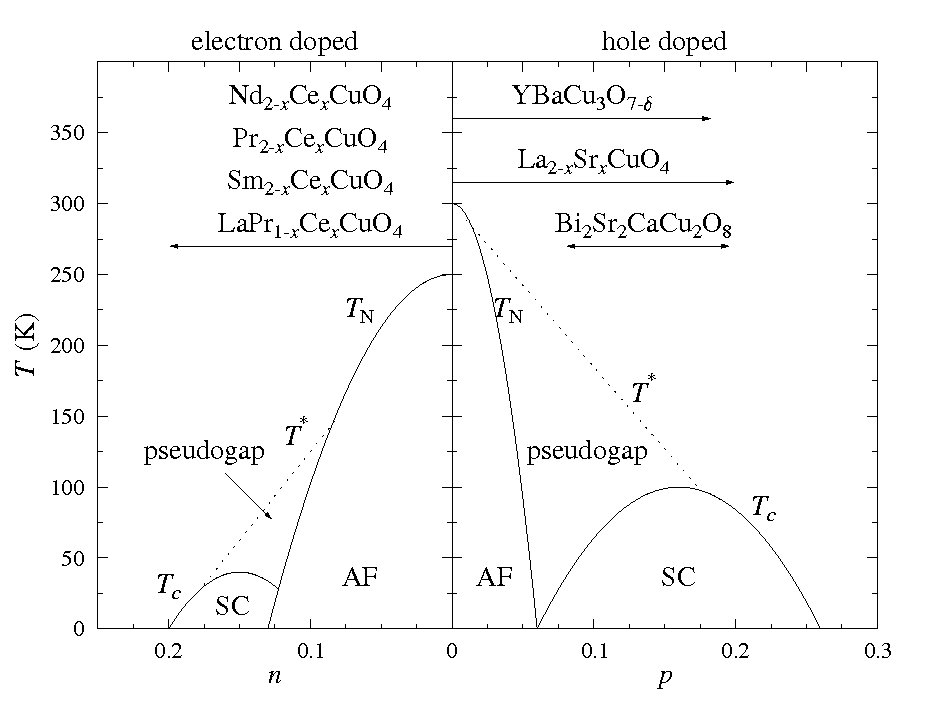
\includegraphics[width=0.8\textwidth]{images/CuPhaseDiag.png}
  \caption[Simplified version of the cuprate superconductor phase diagram]
  {Simplified version of the cuprate superconductor phase diagram \protect\cite{CuPhaseDiag}.}
  \label{fig:CuPhaseDiag}
\end{figure}

Since electrons must be bound together to form Cooper pairs, it was unexpected to find strong electron-electron correlations in copper oxide superconductors. 
One example is given by La$_2$CuO$_4$ which is an insulating material and becomes superconducting, with holes as charge carriers, by replacing some of the trivalent La$^{3+}$ in with the divalent Sr$^{2+}$. 
Band-structure calculations based on the local-density approximation predict the undoped parent compound La$_2$CuO$_4$ to be metallic but it is found to be an antiferromagnetic insulator \cite{Timusk1999}.
This discrepancy is a consecuence of the failure of the independent-particle picture assumed in band-structure calculations and suggests that the undoped parent compounds of the cuprate superconductors are \textit{Mott-Hubbard insulators} \cite{Mott1949}.
That is, the insulating properties are due to strong electron-electron interactions which, nonetheless, allow charge to be bound in Cooper pairs in the superconducting state achieved by doping.

Another remarkable feature of the cuprate high-temperature superconductors is the temperature dependence of the normal state resistivity.
In optimally doped materials resistivity shows a linear variation with temperature from $T_c$ to high temperatures (600-1000K) extrapolating to zero resistance at zero degrees \cite{Gurvitch1987}.
In contrast, conventional metals show a resitivity linearly dependent on temperature only for a limited range of temperatures, have an intercept on the temperature axis at some value grater than zero and saturate at high temperatures \cite{Timusk1999}.
The dependence of the resistivity with temperature is different depending on the doping. 
We provide a more detailed review later in this introductory chapter (section \ref{sec:resistivity}) but we emphasize that these resistivity measurements in the (poor) metal phase of the copper oxides differ from what is expected in a normal (Fermi-liquid\footnote{Fermi-liquid theory describes the excitations in terms of an interacting gas of renormalized quasiparticles.}) metal.
This measurements also indicate a failure of the single-particle picture and suggests the non-applicability of Fermi-liquid theory \cite{Orenstein2000}.

One of the defining properties of a superconductor, within the band energy approximation, is the presence of an energy gap, but early experiments could not find this characteristic signature in cuprate superconductors.
Instead of abruptly finding a zero density of states below a certain energy at the superconducting transition temperature there was only a partial depression of excitations appearing at a much higher temperature $T^*$.
This region in the phase diagram has been called the \textit{pseudogap phase} and there is evidence for its presence in all cuprate superconductor families \cite{Timusk1999,Muller2007}.
Within the band-theory approximation, a \textit{pseudogap} occurs when some regions of the Fermi surface become gapped while other parts remain conductive. 
With increased doping the gapped portion decreases and the compounds become more metallic. 
However, there is evidence that the pseudogap develops smoothly into the superconducting gap and that there are already preformed charge pairs albeit without long range order \cite{Orenstein2000}. 
The pseudogap seems a fundamental property of underdoped copper oxides however, although its relationship to superconductivity still remains unclear, it seems that both phases are intimately related \cite{Basov2005}.

In addition to these peculiarities, cuprate superconductors are instrinsically inhomogeneous systems.
For example in La$_{1.85}$Sr$_{0.15}$CuO$_{4}$ and La$_{2}$CuO$_{4.1}$, the dopant atoms, necessary for superconductivity, do not reside at the crystal symmetric sites making these compounds structurally inhomogeneous \cite{Poccia2011}.
In YBa$_2$Cu$_3$O$_{7-\delta}$ (YBCO) the dopant atoms reside in crystal symmetric positions but the departure from stoichiometry produces compositional disorder \cite{Chen1988,Andersen1990} making YBCO also an inhomogeneous system.
Furthermore, even though the dopant atoms are at fixed positions, these structural inhomogeneities have a dynamical character \cite{Mihailovic2005,Bianconi1996}.
Such a dynamical inhomogeneity is present even in some compounds with perfect crystallographic symmetry like HoBa$_{2}$Cu$_{4}$O$_{8}$ \cite{RubioTemprano2000}.
In addition to the breaking of the crystalline translational symmetry, the pseudogap phase exhibits other broken symmetries. 
The crystalline rotational symmetry is broken locally in La$_{1.85}$Sr$_{0.15}$CuO$_{4}$ with alternating regions of tetragonal and orthorhombic symmetry \cite{Bianconi1996} according to X-ray absorption spectroscopy. 
Time-reversal symmetry breaking was found using angular resolved photoemission spectroscopy with circularly polarized photons in Bi$_{2}$Sr$_{2}$CaCu$_{2}$O$_{8+\delta}$ \cite{Kaminski2002}. 
The clues provided by these broken symmetries should yield an understanding of the ground state in this pseudogap phase, its elementary excitations and the appearance of superconductivity at temperatures below the onset of the pseudogap. 
The existence of these dynamical inhomogeneities suggests that a complete theory of superconductivity is unrechable assuming a perfect crystal structure without consideration for local real-space variations.

Another important aspect to take into consideration is the role of electron-lattice interaction in cuprate superconductors.
One strong motivation for Bednorz and M\"{u}ller to search for superconductivity in Ba$_x$La$_{5-x}$Cu$_5$O$_{5(3-y)}$ was the possibility of strong electron-phonon interactions in oxides due to polaron\footnote{A \textit{polaron} is a quasiparticle formed by correlated movement bewteen a charge carrier and a lattice distortion.}
formation \cite{Bednorz1986}.
Later, X-ray absorption experiments found a large oxygen-isotope effect on the pseudogap onset temperature $T^*$ which is sign reversed with respect to the isotope effect on $T_c$.
It was also found that there were local deviations on the Cu-O bond lengths appearing at $T^*$.
This evidence points to the significance of electron-lattice interactions in the pseudogap phase
In particular the local deviations on the Cu-O bond lengths has been interpreted in terms of polaron formation \cite{MustredeLeon1992}.
Since in a polaronic state the lattice and charge degrees of freedom can not be separated, it is not possible to apply the Born-Oppenheimer approximation \cite{Born1927}.
Thus, for a complete description of cuprate superconductors, it is impossible to separate the ionic and the electronic motions.

The Bardeen-Cooper-Schrieffer (BCS) theory of superconductivity \cite{Bardeen1957} was developed for and successfully applied to metals within the Fermi-liquid approximation. In its current formulation, it seems to lack an appropriate foundation to describe high-temperature superconductivity in copper oxides \cite{Damascelli2003}.
The strong electron-electron correlations prevent accurate band structure calculations assuming independent quasiparticles.
Furthermore the presence of polaronic objects and the observation of lattice and electronic inhomogeneities point to the inadequacy of the Born-Oppenheimer approximation and the reciprocal space formalism.
Such approximations may still remain useful in understanding some aspects of cuprate oxide superconductors but it is clear that there are important features that they are unable to explain.

One approach to explore the electron-lattice dynamics in an inhomogeneous system away from the Born-Oppenheimer (adiabatic) approximation is through model hamiltonians in real space describing both, charge and atomic, degrees of freedom with an appropriate interaction between them.
Unfortunately the computationally resources required to deal with such hamiltonians rapidly increase with each degree of freedom introduced thus making unfeasible to explore large systems with many variables.
As such, we are forced to focus on small subsystems in the copper oxide superconductors.
Since there is strong evidence for polaronic behaviour in the O(4)-Cu(1)-O(4) cluster \cite{MustredeLeon1992,Salkola1994} in the YBCO superconductor it seems essential to correctly describe this subsystem using a non-adiabatic hamiltonian in real space.
Furthermore, some models have considered the interaction between fermionic \textit{pairs} and bipolaronic bosonic objects \cite{Bussmann-Holder2005,Mihailovic2001,Bar-Yam1991,Bianconi2000} explaining several properties of the normal state in the pseudogap region. 
The bipolaronic objects could arise from the O(4)-Cu(1)-O(4) cluster and couple to fermionic carriers on the CuO$_2$ planes thus raising the importance of correctly describing this subsystem.
A particular model hamiltonian has been used to successfully describe the local inhomogeneities and optical signatures in this cluster as a consecuence of polaron formation \cite{MustredeLeon1992, Salkola1994, Salkola1995,DeLeon1999, Leon2008, MirandaMena2007,Mena2006,MustredeLeon2000}.
Although there is a considerable amount of work on this model hamiltonian, the effect of the polaron formation on the \textit{electronic}\footnote{The departure from the Born-Oppenheimer approximation means that the excitations in the model can not be identifyed as having either a lattice or electronic origin but are always in a \textit{mixed} state of both. Thus, when we refer to an \textit{electronic} excitation we mean an excitation that in the absence of electron-lattice coupling would correspond to the electronic degrees of freedom in the model.} excitations of the model has not been throughly explored.
In this thesis we describe in detail this model hamiltonian and many of its lowest excitations incluiding the electronic excitations.
It remains as future work to extend this model to include the coupling of the polaronic objects in the O(4)-Cu(1)-O(4) cluster to superconducting fermionic pairs, although we propose such a model hamiltonian in the conclusions (section \ref{sec:multiSuperc}).

The remainder of this introductory chapter is devoted to reviewing some of the experimental results pointing to the importance of considering the charge-lattice coupling as well as the lattice and electronic inhomogeneities in the description of superconductivity. 
We start, in section \ref{sec:dynamicDistortions} with an overview of the dynamic local lattice and electronic distortions in cuprate superconductors as observed by several experimental techniques. 
In sections \ref{sec:specific_heat} and \ref{sec:resistivity} we present some experimental anomalies in the specific heat and electric resistivity respectively that point to the appereance of a pseudogap and the inapplicability of Fermi-liquid theory.
Finally we discuss some of the experimental results in isotopic effects in section \ref{sec:isotopic_effects} giving evidence of polaronic effects and the need to correctly describe correlated charge-lattice excitations away from the Born-Oppenheimer approximation.


\section{Dynamic local lattice and electronic inhomogeneities}
\label{sec:dynamicDistortions}

All cuprate high-$T_c$ superconductors consist of a given number $n$ of CuO$_2$ planes separated by \textit{charge reservoirs}.
Some materials, such as La$_{2-x}$Sr$_x$CuO$_4$ and Nd$_{2-x}$Sr$_x$CuO$_4$, have one CuO$_2$ plane per unit cell. 
Other compounds like Bi$_2$Sr$_2$Ca$_{n-1}$Cu$_n$O$_{2n+4+x}$ have been synthesized with $n=1,2$ and 3 CuO$_2$ planes per unit cell \cite{Basov2005}.
In this thesis we give particular attention to YBa$_2$Cu$_3$O$_{7-\delta}$ (YBCO) which has two CuO$_2$ layers per unit cell and is one of the most commonly studied compounds.

The crystal structure of YBa$_2$Cu$_3$O$_6$ ($\delta=1$) is tretragonal (\textit{P4/mmm} space group) whereas YBa$_2$Cu$_3$O$_7$ ($\delta=0$) is orthorrombic (\textit{Pmmm} space group).
The oxygen atoms in YBCO occupy four inequivalent positions and are usually labelled as follows: O(1) is in the Cu-O \textit{chains}, O(2) and O(3) are in the CuO$_2$ \textit{planes}, and O(4) is the \textit{apical} oxygen (see Figure \ref{fig:YBCO_structure}).
Each oxygen contributes in a different way to the several properties of the material.
The sites O(2), O(3), and O(4) are always filled whereas, depending on the value of $\delta$, the population of the O(1) sites varies.
The $\delta$ value depends on the growing and treatment conditions, specially on the thermal annealing at different atmospheres or in vacuum \cite{Ivanov1995}.
The two copper atoms in the unit cell also occupy two inequivalent positions.
The labels Cu(1) and Cu(2) are usually assigned to copper atoms in the chains and CuO$_2$ planes respectively.
It is commonly accepted that the Cu(1)-O(1) chains serve as reservoirs for excess holes \cite{Pickett1989}. 
At low $\delta$ the holes are localized at the chains and do not contribute to the conductivity at low temperatures however, at larger $\delta$, a hole transfer occurs to the Cu(2)-O(2),O(3) planes and the samples become superconducting \cite{Cava1988}.

\begin{figure}[ht]
  \centering
  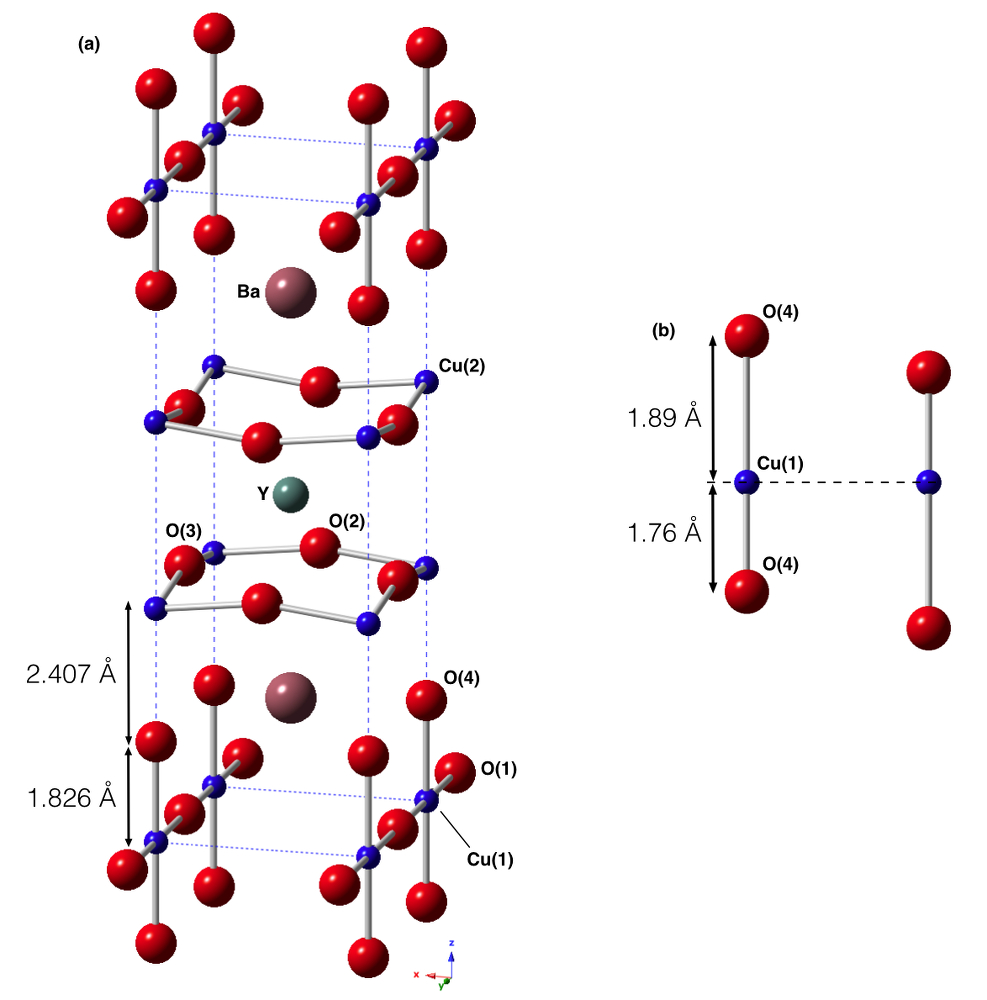
\includegraphics[width=0.7\textwidth]{images/YBCO_O-Cu-O.jpg}
  \caption[Crystal structure of YBa$_{2}$Cu$_{3}$O$_{7}$ and the two possible O(4)-Cu(1)-O(4) configurations.]
  {\textbf{(a)} Crystal structure of YBa$_{2}$Cu$_{3}$O$_{7}$. The dashed line denotes de unit cell. \textbf{(b)} The two possible configurations in the O(4)-Cu(1)-O(4) cluster due to the split O-Cu bond distances (not to scale).}
\label{fig:YBCO_structure}
\end{figure}

Crystal structure in cuprates was determined first by diffraction methods without any sign of significant distortions associated with the in-plane nor with the apical oxygen atoms \cite{Capponi1987,Schafer1988}. 
One of the first observations of a local lattice distortion in cuprates was made using Cu K-edge extended X-ray absorption fine structure (EXAFS) measurements.
It showed a two distances for the Cu(1)-O(4) bond length in YBa$_2$Cu$_3$O$_7$ at temperatures above the superconducting transition temperature, T$_{c}$, with a difference in length close to 0.13 \AA\ \cite{MustredeLeon1990,Conradson1990}.
Since the average bond lengths in diffraction have a significantly higher precision ($\sim 0.001$ \AA\ \cite{Miceli1988}) than local probes like EXAFS \cite{Rehr2000}, these reports were controversial \cite{Kwei1990}.
To resolve the controversy, it was noticed that the time scale in EXAFS measurements is such that dynamical distortions can be measured but, depending on the size of the distortion, elastic techniques like X-ray or neutron diffraction are unable to detect them \cite{Salkola1995}.
For example, it was shown that the two-site O(4) distribution in in Tl$_{2}$Ba$_{2}$CaCu$_{2}$O$_{8}$ could be only detected in a pair distribution function obtained from neutron inelastic scattering, but not with that obtained from neutron diffraction \cite{Egami1991}. 
Consequently, it is important to take into account both the spatial resolution and time resolution of the techniques used to study the actual atomic structure of these materials \cite{Mihailovic2005}. 
The explanation of the discrepancies between these results with diffraction and optical spectroscopical results lead to the interpretation of this two-sites Cu(1)-O(4) distribution as a dynamical distortion of polaronic origin \cite{MustredeLeon1992}.

In YBa$_2$Cu$_3$O$_7$ the EXAFS analysis using polarized X-rays on magnetically oriented powders showed two different Cu(1)-O(4) distances diferring by $\sim 0.10-0.13$ \AA\ that changed into a single site distribution in the vicinity of the superconducting transition temperature \cite{Conradson1990,MustredeLeon1992a}. 
This result was also received with skepticism based on earlier diffraction \cite{battlog1992lattice,Kwei1990,Sharma1991} and optical spectroscopy \cite{Thomsen1993} results. 
However, independent EXAFS measurements in other oriented samples \cite{Stern1993} and single crystals \cite{Booth1996} also showed a two-site distribution in YBa$_{2}$Cu$_{3}$O$_{6.7}$, YBa$_{2}$Cu$_{3}$O$_{6.5}$ and Co doped  YBa$_2$Cu$_{2.8}$Co$_{0.2}$O$_{7+\delta}$ \cite{MustredeLeon1991}. 

Similar two site distributions obtained from EXAFS spectra were found for the Cu(2)-O(4) distribution in Bi$_{2}$Sr$_{2}$CaCu$_{2}$O$_{8}$ \cite{bianconni1992lattice} and in TlBa$_{2}$Ca$_{3}$Cu$_{4}$O$_{11}$ \cite{Allen1991} starting at temperatures above T$_{c}$. 
In these compounds (and other cuprates) the average Cu(2)-O(4) bond length lies between 2.49 and 2.73 \AA, which is much longer than the Cu(1)-O(4) bond length in YBa$_{2}$Cu$_{3}$O$_{7}$ ($\sim 1.87$ \AA). 
This fact makes more difficult the identification of details about the O(4) distribution due to the stronger mixing of the Cu(2)-O(4) EXAFS signal with those of other atoms and the increased zero point motion of the O(4) atom due to weaker Cu(2)-O(4) bond compared with the Cu(1)-O(4) bond.
For this reason in most EXAFS studies addressing the O(4) motion a gaussian single site broadened distribution has been used, reporting only changes in the width of the distribution as a function of temperature \cite{Booth1995,Oyanagi2007,Zhang2009}.

In plane Cu(2)-O local lattice distortions were identified in La$_{1.85}$Sr$_{0.15}$CuO$_{4}$ appearing below 100 K \cite{Bianconi1996,Oyanagi2007}, in TIBa$_{2}$CuO$_{6}$ below 120 K \cite{Conradson1997} and in La$_{2}$CuO$_{4.1}$ below 150 K \cite{Lanzara1997,MustredeLeon:xj5003}. 
In this case the observation of such distortions in YBa$_{2}$Cu$_{3}$O$_{7}$ and related compounds becomes more difficult due the similarity in Cu-O bond lengths in the CuO$_2$ planes and chains, whose contributions are mixed in the EXAFS signal \cite{Conradson1997,MustredeLeon1992a}.

As of now, only in La$_{1.85}$Sr$_{0.15}$CuO$_{4}$ has been possible to identify local lattice distortions involving both in plane oxygen and apical oxygen atoms  \cite{Bianconi1996}. 
We also stress that from all these EXAFS experiments it is only possible to probe with enough detail the nearest neighbor environment around the Cu atoms, thus the spatial extension of the distortions cannot be determined solely from these measurements. 
Additional structural information \cite{Bianconi1996a} is needed to formulate models about the extension of the distortions as discussed in Ref.\ \cite{Bianconi1996}.
Pair distribution function analysis of X-ray diffraction, X-ray and neutron inelastic scattering can additionally provide information about the intermediate range (up to 10-15 \AA) atomic structure, complementary to the information obtained from EXAFS \cite{Egami2003}. 
Pair distribution function results in La$_{1-x}$Sr$_{x}$CuO$_{4}$ \cite{Bozin1999,Bozin2000} indicate that the atomic structure in this material is a combination of nanoscale regions with different local Cu-O environments, in agreement with the model proposed in Ref.\  \cite{Bianconi1996}. 
A homogeneous structure only appears when dopant concentrations are above $x = 0.25$. 
In this region the electronic behavior can be described in terms of free fermion quasiparticles.

Although an inhomogeneous electronic ground state does not necessarily follow from structural inhomogeneities, such as the ones discussed in the previous section, for some regions of the phase diagram such state is realized.
Early EXAFS analysis in La$_{1.85}$Sr$_{0.15}$CuO$_4$ and X-ray diffraction in Bi$_2$Sr$_2$CaCu$_2$O$_{8+y}$ showed two orders of the CuO$_6$ octahedra below 100K assigned to two types of \textit{stripes} with different order, one of them with a large tilting and elongation of the in-plane Cu-O distances.
This significant distortion was taken as an indicative that the electronic structure in both kind of stripes is different \cite{Bianconi1996,Bianconi1996a}.
Since then it has been possible to detect the existence of srtipe-ordered phases in La$_2$CuO$_{4+\delta}$, La$_{1.6-x}$Nd$_{0.4}$Sr$_x$CuO$_4$, La$_{2-x}$Ba$_x$CuO$_4$, La$_{2-x}$Sr$_x$CuO$_4$ \cite{Kivelson2003}, Bi$_2$Sr$_2$CaCu$_2$O$_{8+\delta}$ \cite{Poccia2011a} and YBa$_2$Cu$_3$O$_{7-\delta}$ \cite{Mook2002,Haase2003}.
Spatial variations in the densitiy of states (stripes) have also been measured using scanning tunneling miscroscopy (STM) \cite{Pan2001} and angle-resolve photoemission spectroscopy (ARPES) \cite{Salkola1996}. 

\section{Specific heat}
\label{sec:specific_heat}

Specific heat ($C$) measurements in bulk superconductors can provide useful information about the superconducting and normal states.
Important quantities for the conventional theory of superconductivity, such as the density of electronic states at the Fermi energy and the Debye characteristic temperature, can be obtained from specific heat measurements below $T_c$ in a magnetic field exceeding the upper critical field ($H_{c2}$), that is, with superconductivity supressed.
The densitiy of states at the Fermi energy can be obtained from the linear term ($\gamma T$) of the specific heat while the Debye characteristic temperature can be obtained from the $T^3$ term.
The specific heat comprised of the odd polynomial terms is the \textit{lattice} part ($C_l$) and gives some information about phonon dispersion. 
The electronic specific heat in the superconducting state  ($C_{es}$) can be obtained by subtracting $C_l$ from zero-field measurements.
The discontinuities in $C$ at $T_c$ and $C_{es}$ are related to the magnitude of the electron-phonon coupling in conventional BCS superconductors.
Thus the temperature dependence of $C_{es}$ might show evidence of certain different mechanisms of superconductivity, although some non-BCS mechanisms could give the usual BCS result.

Unfortunately, for cuprate superconductors there are several problems hindering the analysis of specific heat experiments.
One of them is that $T_c$ typically occurs in temperature regions in which $C_l$ is about a hundred times larger than other contributions and has a complicated temperature dependence.
Another problem arises from the fact that the upper critical fields $H_{c2}$ are usually too large to supress superconductivity and obtain normal-state information except at temperatures close to $T_c$.
Also, there are magnetic impurities that complicate the interpretation at low temperatures \cite{Fisher1988}.

Nevertheless, electronic specific heat was successfully measured using a differential techinque comparing a superconducting sample with a very similar non-superconducting sample. 
Although some corrections have to be made due to the change in phonon spectrum between samples, the electronic specific heat can be largely determined by this method \cite{Loram1990,Loram1993, Loram1994}.
An ensuing investigation of the electronic specific heat of Y$_{0.8}$Ca$_{0.2}$Ba$_2$Cu$_3$O$_{7-\delta}$ as a function of oxygen doping ($0.04\leq \delta \leq 0.89$) showed very different behaviours for the electronic specific heat coefficient $\gamma (T) = C/T$ in the underdoped ($\delta > 0.32$) and overdoped ($\delta < 0.32$) samples \cite{Loram1997}.

In the overdoped samples, (see FIG 2 (a) from \cite{Loram1997}), $\gamma (T)$ is temperature independent if the sample is in its normal state.
Since for a Fermi liquid the specific heat rises linearly with the temperature (i.e. $\gamma (T)$ is constant) this suggests that the overdoped sample is similar to a normal metal. 
At $T_c$ there is a specific heat jump which is larger than what is expected for a BCS model assuming a weak coupling suggesting that superconductivity in copper oxides is driven by strong couplings.

In the underdoped samples there is a plateau where $T_c$ varies slowly but there is a sudden decrease in the height of the specific heat jump at $T_c$.
In these underdoped samples there is a depression of $\gamma (T)$ in the normal state which is interpreted as a consequence of a pseudogap. 
This depression starts at higher temperatures when more oxygen is removed.
There has been similar evidence of a pseudogap in the normal state for some more hole-doped cuprates \cite{Loram2001}.


\section{Electric resistivity}
\label{sec:resistivity}

In conventional (Fermi-liquid) metals the electric resistivity, $\rho(T)$, at low temperatures is a linear function of temperature intercepting the temperature axis at some point and saturating at high temperatures.
In contrast, the electric resitivity in optimally doped copper oxide superconductors was found to be a linear function of temperatures for a wide range $\sim 10-1000$ K and extrapolates to zero resitivity at zero degrees \cite{Timusk1999,Muller2007}.
In the underdoped materials there is a break in the slope of this linear behaviour at a temperature near the pseudogap onset temperature $T^*$ as observed by nuclear magnetic resonance \cite{Bucher1993}.

The doping dependence of the electric resistivity in the ab-plane, $\rho_{ab}(T)$, which is parallel to the CuO$_2$ planes, is qualitatively different in the underdoped and overdoped compounds.
For the underdoped samples, at low temperatures $\rho_{ab}(T)$ shows \textit{semiconducting} behaviour with the resistivity decreasing with temperature down to a minimum before increasing again superlinearly up to $T^*$ where a break in slope makes $\rho_{ab}$ approximately linear \cite{Timusk1999}.
In the overdoped samples the resistivity shows an approximately linear dependence with $T$ \cite{Damascelli2003} similar to the Fermi-liquid behaviour, however this linear behaviour extends to much higher temperatures than expected and there are many other properties that do not follow the expected Fermi-liquid behaviour \cite{Orenstein2000}.

These measurements show both the inapplicability of Fermi-liquid theory to the copper oxides and the presence of a pseudogap in the underdoped samples.

\section{Isotopic effects}
\label{sec:isotopic_effects}

The effect of isotopic substitutions was important in the understanding and validation of BCS superconductivity.
This effect manifests itself as a change in the superconducting transition temperature ($T_c$) with the ionic mass ($M$) in the form $T_c \propto M^{-\alpha}$ where $\alpha$ is called the \textit{isotope coefficient}.
In the simplest case of a monoatomic lattice in a BCS superconductor it takes the value $\alpha=0.5$.
The observation of this isotope effect \cite{Reynolds1950,Maxwell1950} was evidence of the crucial role played by the electron-lattice interaction in the formation of Cooper pairs. 
In complex materials, such as the cuprate superconductors, there are many factors that can affect the value of the isotope coefficient, such as the presence of several ions, lattice anharmonicity, inhomogeneities and polaronic effects.
All these factors complicate the interpretation of the isotope effects observed in cuprates.

The isotope effect and its temperature dependence has been extensively studied in copper oxides.
Its behaviour is very different from what can be expected for a simple BCS supercondcutor.
In particular, YBCO allows a site-selective substitution $^{16}$O $\rightarrow$ $^{18}$O enabling a precise study of the isotopic effect for each different oxygen site \cite{Conder1993,Cardona1988}. 
At optimal doping $\alpha$ was observed to be relatively small \cite{Thomsen1988}, however it grows significantly by reducing the doping level \cite{Bishop2007}.
Making site-specific substitutions and measuring the changes in the phonon frequencies  allowed a differentiation of the contributions of the different ions.
It was found that the (small) isotope effect on $T_c$ mainly comes from in-plane oxygens with little contribution from the apical oxygen  \cite{Ruani1994,Zech1994}.
Since the superconducting charge carriers reside in the CuO$_2$ planes, this suggests a fundamental role of the lattice dynamics in the superconducting state.
Also, it was found that the \textit{harmonic} approximation accounts well for the O(2)/O(3) vibrations but it fails for O(4) \cite{Ruani1994}.

Another observable quantity that shows an isotope effect is the London penetration depth $\lambda_L$.
At optimum doping, in contrast to what is observed for $T_c$, the isotope effect is rather large in $\lambda_L$ and it similarly increases with a decrease in doping \cite{Zhao1997,Hofer2000,Khasanov2004}.
It should be noted that in a conventional BCS superconductor the isotope effect on $\lambda_L$ is zero.
Similarly for the two-gap superconductor MgB$_2$, in which superconductivity is mediated by electron-phonon interactions, there is no isotope effect in $\lambda_L$ \cite{Castro2004}.
This isotope effect in cuprate oxides further suggests that the ionic lattice and the electron-lattice interaction are fundamentally involved in the appearance of superconductivity in these compounds \cite{Kresin2009}.
It even has been argued that from the isotope effects in the London penetration depth follows that the carriers are polaronic objects with an oxygen-isotope dependent in-plane effective supercarrier mass \cite{Zhao1997,Hofer2000,Khasanov2004}.

Another isotope effect was found on the pseudogap onset temperature $T^*$ using two different experimental techniques, EXAFS and inelastic neutron scattering, in the La$_{1-x}$Sr$_x$CuO$_4$ and HoBa$_2$Cu$_4$O$_8$ compounds \cite{Lanzara1999,RubioTemprano2000}.
These experiments show a very large isotope effect that is sign-reversed with respect to the effect on $T_c$.

Lastly, there is a report of a large isotope effect in the electronic structure on optimally doped Bi$_2$Sr$_2$CaCu$_2$O$_{8+\delta}$ samples measured by ARPES. 
This was interpreted in terms of a significant pairing between electrons and the ionic lattice with the magnitude of the effect correlated with the pair binding energy \cite{Gweon2004}.
However, a later study failed to find such large isotope effect \cite{Douglas2007} in the same compound.
To our knowledge this controversy still remains unresolved.
In the present work, in section \ref{sec:elIsotShift}, we find an isotope effect in the electronic structure of YBa$_2$Cu$_3$O$_{7-\delta}$ under an oxygen isotope substitution \cite{GarciaSaraviaOrtizdeMontellano2014}.
However we are still lacking a clear interpretation of our results in terms its measurable effects on ARPES measurements preventing us to draw a significant conclusion at the moment.

Aditionally, it should be noted that isotopic shifts have been used to identify particular excitations in infrared and Raman spectra as phononic in origin (v.g. \cite{Thomsen1990}) however, as we will discuss in section \ref{sec:irIsotopicShifts}, in the case of the apical oxygen, due to polaronic effects, a \textit{phononic} excitation could have an isotope effect very close to zero.
